\chapter{Kinetic formulation and numerical controls}\label{ch:numerics}
\section{Distribution functions and statistical particles}
For species $s$, let $f_s(\boldsymbol{x},\boldsymbol{v},t)$ be number density
in phase space. A representative kinetic equation is
\begin{equation}
\frac{\partial f_s}{\partial t}+\boldsymbol v\cdot\nabla_x f_s+
\frac{\boldsymbol F_s}{m_s}\cdot\nabla_v f_s
=C_s[f]+S_s-L_s .
\end{equation}
Which terms are present depends on the application. Neutral DSMC, test-particle
transport and self-consistent electromagnetic PIC use different closures;
they are not interchangeable run modes obtained by changing one rate.

A macroparticle $p$ represents $w_p=W_{s,b}c_p$ physical particles, where
$W_{s,b}$ is the selected base weight (possibly block-local) and $c_p>0$ is
an enabled individual correction. Fixed-weight configurations use the
corresponding compiled convention. A weight is a physical multiplicity,
not a particle mass and not an arbitrary plot normalization.

In cell volume $V$, instantaneous estimators are
\begin{align}
n_s&=\frac{1}{V}\sum_{p\in s}w_p,&
\boldsymbol u_s&=\frac{\sum w_p\boldsymbol v_p}{\sum w_p},\\
\mathsf P_s&=\frac{1}{V}\sum_{p\in s}w_p m_s
(\boldsymbol v_p-\boldsymbol u_s)(\boldsymbol v_p-\boldsymbol u_s)^T,&
T_s&=\frac{\operatorname{tr}\mathsf P_s}{3n_s k_B}.
\end{align}
The three-dimensional temperature formula applies to three translational
velocity degrees of freedom. A DIM1 spatial mesh does not automatically
remove transverse velocity components. A surface flux estimator instead
uses crossing weight divided by area and physical accumulation time.

\begin{figure}[htbp]
\centering
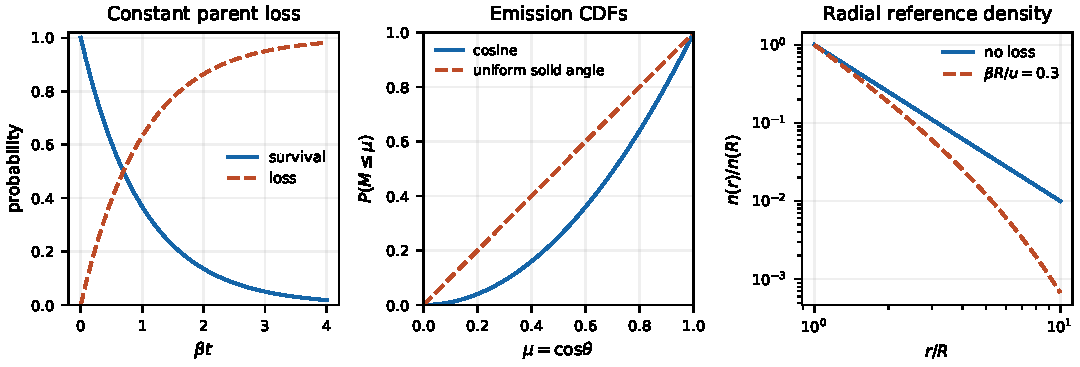
\includegraphics[width=\linewidth]{figures/kinetic_reference.pdf}
\caption{Independent analytical limits, not simulation results. Left: constant
first-order parent loss. Centre: outgoing cosine-law and uniform-solid-angle
CDFs in the normal-direction cosine. Right: steady spherical constant-speed
outflow, $n(r)/n(R)=(R/r)^2\exp[-\beta(r-R)/u]$, excluding gravity, collisions,
returning particles and distributed sources. These limits illustrate different
normalization and physical assumptions; they are not universal coma solutions.}
\label{fig:reference-limits}
\end{figure}

\section{Time step, mesh resolution and particle weight}
A common transport constraint for a global step is
\begin{equation}
\Delta t\leq \min_{s,b,d}
\frac{C_s h_{b,d}}{v_{\mathrm{char},s}},
\qquad 0<C_s\leq 1 ,
\end{equation}
with cell lengths $h_{b,d}$ in metres and speed in metres per second.
This is an application-selected characteristic-speed bound, not a guarantee
against the tail of a Maxwellian. Gyromotion, field variation, chemistry and
collision accuracy can impose stricter limits. Log actual minimum cells and
the final accepted step, not just the requested resolution.

For a constant physical source $Q_s$ and an expected $N_s$ numerical
injections per step, $W_s=Q_s\Delta t/N_s$ when all particles use one weight.
For a source with acceptance/rejection, local time steps or importance
sampling, derive the represented \emph{accepted} rate and its correction
instead of applying that expression blindly.
For local face transfer the represented crossing rate is $Wc/\Delta t$.
The opt-in resampling multiplicity is
\begin{equation}
\mu_{\rm face}=\frac{W_{\rm old}\Delta t_{\rm new}}
{W_{\rm new}\Delta t_{\rm old}} .
\end{equation}
The individual correction cancels only under the implemented policy of
holding that correction fixed. Continuation across MPI owners must finish
before sampling or generic splitting can duplicate an unfinished trajectory.

\section{Choosing a discretization for DSMC}
Resolve the shortest relevant density/temperature/flow scale and assess cell
size relative to mean free path. Separate transport and collision time errors.
For a dilute single-species estimate,
$\lambda\sim1/(\sqrt{2}n\sigma)$; mixtures and speed-dependent cross sections
require an appropriate collision integral. Refine where collisional and
surface gradients are strongest, then demonstrate convergence of the
actual observable. Increasing particles alone does not remove mesh bias.

Representative counts per collision cell must support the selected pair
algorithm. Sparse cells can have biased or noisy rates even when the total
particle population is large. A large sample window does not remedy a
systematic collision-cell or trajectory error.

\section{Sampling, stationarity and uncertainty}
Discard startup transients based on relaxation/transport times and observable
histories, not an unexplained iteration count. A sampling length in steps
corresponds to $N_{\rm sample}\Delta t$ only for a fixed global step.
Retain the actual physical accumulation interval for variable-step estimators.
Estimate uncertainty using independent realizations or block averages long
enough to expose autocorrelation. The familiar $N^{-1/2}$ statistical scaling
does not justify treating correlated stored samples as independent.

Separate three studies: mesh refinement at controlled statistics, timestep
refinement at controlled mesh, and particle/sample refinement at fixed
discretization. Include boundary-distance and external-data resolution studies
when those control the observable. Never fit a source with one numerical
error and interpret the compensation as a measured physical rate.

\section{Random streams and population control}
Record seed, rank/thread layout and stream policy. Reproducibility on the
same layout does not imply identical particles after repartitioning.
For a constant Poisson rate $\nu$, sample
$\tau=-\log(1-u)/\nu$ with the generator's declared endpoint convention.
Numerically \code{-log1p(-u)} resolves small $u$ well; replacing the draw by
\code{-log(u)} changes a fixed seeded path even though both have the same
continuous distribution.

Generic split/merge must preserve the moments required by the application,
and must specify what happens to opaque extension bytes. Conserving number,
momentum and scalar energy does not preserve all angular or higher moments.
Dust requires its own size-sensitive rules (Chapter~\ref{ch:dust}).
\source{src/pic/README.md; test/srcCoreUnitTests/README.md}
